
%----------------------------------------------------------------------------------------
%	PACKAGES AND OTHER DOCUMENT CONFIGURATIONS
%----------------------------------------------------------------------------------------

\documentclass[12pt]{article} % Default font size is 12pt, it can be changed here
\usepackage{hyperref}
\usepackage{amsmath}
\usepackage{geometry} % Required to change the page size to A4
\geometry{a4paper} % Set the page size to be A4 as opposed to the default US Letter

\usepackage{graphicx} % Required for including pictures

\usepackage{float} % Allows putting an [H] in \begin{figure} to specify the exact location of the figure
\usepackage{wrapfig} % Allows in-line images such as the example fish picture

\usepackage{lipsum} % Used for inserting dummy 'Lorem ipsum' text into the template

\linespread{1.2} % Line spacing

%\setlength\parindent{0pt} % Uncomment to remove all indentation from paragraphs

\graphicspath{{./Pictures/}} % Specifies the directory where pictures are stored
\begin{document}

%----------------------------------------------------------------------------------------
%	TITLE PAGE
%----------------------------------------------------------------------------------------

\begin{titlepage}

\newcommand{\HRule}{\rule{\linewidth}{0.5mm}} % Defines a new command for the horizontal lines,
%change thickness here
\center % Center everything on the page

\includegraphics[width=\textwidth]{Glasgow}\\[1.5cm]
\textsc{\LARGE Human Computer Interaction 4}\\[0.5cm] % Major heading such as course name
\textsc{\Large Assessed Exercise}\\[0.5cm] % Minor heading such as course title

\HRule \\[0.4cm]
{ \huge \bfseries Hide and Seek Mobile Application}\\[0.4cm] % Title of your document
\HRule \\[1.5cm]

\begin{minipage}{0.4\textwidth}
\begin{flushleft} \large
\emph{Author:}\\
Garry \textsc{Sharp}\\
0801585s\\ % Your name
\end{flushleft}
\end{minipage}
~
\begin{minipage}{0.4\textwidth}
\begin{flushright} \large
\emph{Supervisors:} \\
Prof. S. \textsc{Brewster}\\ % Supervisor's Name
Dr. M. \textsc{Chalmers}\\ % Supervisor's Name
Dr. A. \textsc{Morrison}\\ % Supervisor's Name
\end{flushright}
\end{minipage}\\[4cm]

{\large \today}\\[3cm] % Date, change the \today to a set date if you want to be precise

\vfill % Fill the rest of the page with whitespace

\end{titlepage}

%----------------------------------------------------------------------------------------
%	TABLE OF CONTENTS
%----------------------------------------------------------------------------------------

\begin{abstract}
The main inspiration for the system stemmed from an idea, or rather a musing, I had regarding how
difficult and strange it looks to navigate around a space whilst constantly looking at your phone.
Not only does it look strange, it can also be incredibly inconvenient if you do not have both hands
free or are engaged in some other activity such as running. The idea immediately interested me,
and, whilst there were already existing applications to solve these practical issues, the idea of
using multi-modal feedback in map based applications stayed with me. Eventually I opted for a hide
and seek app (See Section \ref{Overview}) which would allow users to experience non-visual
navegation in a fun way.
\end{abstract}
\newpage
\tableofcontents % Include a table of contents

\newpage

\section{System Analysis}

\subsection{Brief Overview and Description of the System}
\label{Overview}

The system is, as the name suggests, a reinvention of the common childrens "Hide and Seek" game. In
a traditional game of hide and seek, the person who is to do the seeking (the seeker) counts to
twenty while the other participant (the hider) uses this time to hide. The seeker then exclaims
"here I come, ready or not" and the game is over when the seeker has found the hider. Another
similar game is called Marco Polo, where the seeker (who has their eyes closed) shouts "Marco" and
the hider responds "Polo", the seeker must then try to catch the hider based on acoustics. The
application that has been developed is a fusion of both of these classic games that runs over a
network, with the hider sending the seeker GPS co-ordinates corresponding to their location and the
seeker then receiving feedback every 60 seconds in the form of vibration pulses and beeps to
indicate if their current bearing and distance in relation to the hider.

\subsection{Aims of the System}
\label{Aims}
The key aim of the system is to provide a fun and interesting way of navigating around a space such
as a park without using any visual aids. The system is designed to accomplish two things, firstly,
provide a new and interesting way of navigating without the use of any visual interface, and
secondly, provide a challenge to the user (in the context of a hide and seek game) to find a peer
with another GPS enabled mobile device. Hopefully the user will also experience similar levels
of cusiosity and intrigue as I did whilst developing it.


\subsection{Purpose of the System} 
The system's primary purpose is to provide entertainment value to its users. Initially the idea was
only concerning navigation without a visual aid, which may have had a useful application in
developing map based applications for the blind or visually impaired, however, there are already
many apps out there that tend to these needs (See Similar Systems below) and so the reapplication of
the technology in a fun way quickly formed itself as the main goal of the system.

\subsection{Similar Systems} 

There are many map based applications on the android market today, perhaps the most well known of
all is google maps, 


%----------------------------------------------------------------------
\newpage
\section{Design and Testing}
The design of the system was focussed primarily on the user interface, this was especially
interesting as I was very adamant not to user traditional visual methods. A series of techniques
were used in the system design and testing which are detailed below, these included, but were not
limited to, the use of Neilsen's heuristics and practical user testing.

\subsection{Design}

The system was designed adhereing to, and in accordance with Nielsen's heuristics (See Section
\ref{Neilsen}). These essentially are a set of commonly agreed upon principles that should be
adhered to when thinking about the design of a user interface. In past project, I used Neilsen's
heuristics in the design of GUIs for various applications, however, this was the first time in
which I applied the heuristics to system that would have no kind of graphical interaction. A
complete description of the heuristics in the hide and seek app can be found below.

\subsubsection{Nielsen's Heuristics}
\label{Neilsen}
\begin{description}
\item[Visibility of system status] \hfill \\
The user should always be informed about what is happening throughout the systems execution, this
is difficult to adhere to in its entirity as part of the app is based explicitly on the user not
knowing whether or not they are going in the right direction. As the app is a game, this is
generally accepted as the goal is to make the location of the person with the broadcasting of the
device intentionally challenging (though not too difficult as to aggrevate the user). The user is
given multi-modal feedback in a number of 10 second windows which I found with user testing (See
Section \ref{Testing}) provided a good balance vis-a-vis challenge and easy navigation.


\item[Match between system and the real world] \hfill \\
This is perhaps the heuristic that was deviated from the most, the user feedback received is very
non-intuitive, however, as a heuristic of convenience (and with the system trying to achieve a level
of inconveniece in not making it too easy to locate someone), I thought it acceptable to deviate
from the traditional convention.

\item[User control and freedom] \hfill \\
The interaction between the user and the system is mostly one sided, that is to say, there is very
little input that the user gives the system (in fact there is no direct input, simply the changed
co-ordinates and direction which is collected as the user moves), contrasted to a large amount of
feedback that is given back to the user. Their position directly influences how the system gives
feedback. The user, however, has no control over the intervals with which feedback is given
(hardcoded system constant). In future development (See Section \ref{FurtherDevelopment}),
intervals of time may be user chosen to reflect varying levels of difficulty.

\item[Consistency and standards] \hfill \\
The vibrate function of the app is only ever used to indicate direction and the beeping sound is
only ever used to indicate difference, in this regard it is very difficult for a user to become
confused after learning what the feedback means.

\item[Error prevention] \hfill \\
The most common error in the system is that it will not work if there is not GPS signal, this makes
use of the app indoors or in built up or wooded areas impossible. Occationaly the system experiences
performace difficulties depending on the quality of the GPS installed on the device. These are the
only known errors and flaws that the system presents.

\item[Recognition rather than recall] \hfill \\
Other than the understanding of the beep/vibrate frequencies (solid = right direction/close,
intermittent = sideways direction/halfway there, no response = totally wrong direction/furthest
away), there is no information that the user needs to remember.

\item[Flexibility and efficiency of use] \hfill \\
This does not apply to this applcation as it is both a game and also requires such little input
from the user that the use of accelerators would be un-necessary.

\item[Aesthetic and minimalist design] \hfill \\
There is not visual display (with the exception of printing error message to the screen), and
therefore, no requirement to worry about aesthetic.

\item[Help users recognize, diagnose, and recover from errors] \hfill \\
Lack of GPS or a weak GPS signal are the only known errors of the system, a message will appear on
the screen informing the user to check that their GPS is turned on or to wait for incoming GPS data
respectivey.

\item[Help and documentation] \hfill \\
A welcome dialogue is displayed upon launching the system informing the users of what a vibration,
beep and the frequencies between them means. As the system is quite lightweight further
documentation would be irrelevant.
\end{description}


\subsubsection{HAPTIMAPS Toolkit}
HAPTIMAPS is an open source toolkit which allows developers to simply and easily create
applications that offer multi-modal feedback for map based applications. Having previously used the
HAPTIMAPS toolkit, I can vouch for its effectiveness and authenticity. This, in fact, was one of
the primary reasons that I decided against its usage in the final system. As native android
provides sufficient functionality for handling GPS data, it was not necessary to include the
HAPTIMAPS toolkit, however, should the app be expanded further (See Section 
\ref{FurtherDevelopment}) I would almost definitly opt to use the toolkit
\subsection{Testing}
\label{Testing}

There were two main testing methodologies employed in the testing of the system, the component
testing (which focussed on whether they system worked), and the acceptance testing (which tested
the systems usability as well as whether it met its goals or not, See Section \ref{Aims}). Both
methodologies are documented and detailed below.

\subsubsection{Unit Testing}

All unit testing strategy comprised of a hybrid of IEEE standard automated tests and manual testing
of the more important components of the system (chiefly the timing, vibrating, beeping and GPS
related functions). Unit testing was performed exhaustively until it met a suitable standard. The
key problem I found was that in the many locations I tested the app, there wasn't always a strong
GPS signal which caused further delays in the system giving feedback. This is also reflected in the
user testing (See Section \ref{Acceptance}).
\subsubsection{Acceptance Testing}
\label{Acceptance}

The acceptance testing was all end user based, a number of peers from the course obliged in a short
testing of the system which took place just outside the Boyd Orr building. The were asked to use
the app for a short time and then report back after a minute as to which direction that would start
walking in if it were 

\begin{table}[h]
\begin{center}
\begin{tabular}{p{0.3\textwidth} p{0.2\textwidth}}
Direction & Percentage \\
\hline\\
Correct Direction & 40\% \\
Slight Discrepency & 40\% \\
Large Discrepency & 20\% \\
Wrong Direction & 0\% \\
\end{tabular}
\caption{Showing accuracy of users after a minutes use}
\label{UserTestResults}
\end{center}
\end{table}

From Table~\ref{UserTestResults} we can see that 80\% of users were able to establish an either
perfectly correct, or roughly correct position (slight discrepency in the table above refers to a
difference of 30$^\circ$ in either direction, whereas large discrepency refers to 30$^\circ$ to
90$^\circ$ in either direction and wrong direction refers to anywhere further than the 90$^\circ$ in
either direction).

\begin{table}[h]
\begin{center}
\begin{tabular}{p{0.3\textwidth} p{0.2\textwidth}}
Position & Percentage \\
\hline \\
Would use the app & 90\% \\
Would not use the app & 10\% \\
\end{tabular}
\caption{Showing accuracy of users after a minutes use}
\label{UserTestUse}
\end{center}
\end{table}

From Table~\ref{UserTestUse} we see very encouraging results related to the popularity of the app
as an overwhelming majority of testers would use the app. However, even though these numbers work
very nicely in favour of the app, the accuracy is questionable, as the app solves no major issues
and merely provides entertainment value, the responses may not have been as honest and
significantly fewer people may actually use the app more than a few times, however, this is to be
expected. 

Overall these were relatively positive figures, it should be noted that the 20\% that failed to
report an accurate direction also suffered GPS issues on their devices as the feedback reveived
indicated that they were indeed facing in the right direction.

\newpage
\section{More Information}
\subsection{Working with new Modalities}

The challenge of working with new modalities was a fun prospect, what added to this was that I was
adament not to use any kind of visual display or feedback, in fact, for the majority of the
implementation stage I kept the android default "Hello World" display (this changed as I now put a
message here if the GPS is not activated). Android offers reasonably good support for accessing the
native vibrate and GPS functions of the mobile device. This meant that applying the application
logic to the vibrate and beep features was relatively straightforward.


\subsubsection{Working with GPS}

One of the initial concerns I had with the system was that of the GPS. Having never used the system
before (accompanied by a limited understanding of how GPS actually works), I did not feel like I
was in the best position to start developing an application that relied heavily upon it. \\

\begin{wrapfigure}{l}{0.5\textwidth} % Inline image example
 \begin{center}
    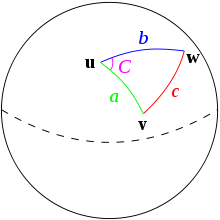
\includegraphics[width=0.42\textwidth]{haversine}
  \end{center}
  \parbox{0.45\textwidth}{\caption{The haversine formula calculating the true distance on the
spherical earth}}
\end{wrapfigure}

After researching the topic, I quickly discovered that many GPS based systems rely heavily upon
maths that is not included as standard in the Java GPS libraries. One such example of this is the
haversine formula which solves the issue of GPS triangulation not giving the true distance between
two points. In reality this is only relevant when calculating distances which are realistically
subject to variation in relation to the curvature of the earth. For instance, calculating distances
over a city would provide a negligable discrpency when constrasting the distances gathered using
the haversine formula with distances caluculated without using it. For this reason, the application
that I have developed does not perform any complex maths using the haversine formula or any other
geo-positioning equations. However, should the app be developed further and used over a larger
geographical scale, then the app would almost certainly have to feature GPS related maths.

\subsection{Further development}                                                                   
\label{FurtherDevelopment}           
Although the system itself was reasonably simple to implement, especially when faking (to an extent)
some of the back end functionality. What is more interesting here is the broader application of the
multimodal feedback that is received whilst using the app. As the user of a broader system would
only have limited interaction with a GUI, the importance would then be placed on having a system
that accurately conveys meaningful messages via vibration and audio. Currently the feedback
received is of a binary nature, that is to say, in the determination of distance or direction you
judge your accuracy by the presence or lack of a beep/vibration. Currently, it is the intervals
between the beeps and vibrations that indicates to the user their direction and distance. The
initial reason for not providing alternative forms of feedback (for instance different intensity of
vibrations or different audio signals), was that the primary purpose of the app is that of a game.
However, similar systems such as HAPTIMAPS (see above section) allow for users to use a series of
common HCI interactivity modes to give feedback to users using map based applications where the
user cannot see the screen.

\newpage
\section{Conclusion} % Major section

%----------------------------------------------------------------------------------------
%	BIBLIOGRAPHY
%----------------------------------------------------------------------------------------

%\begin{thebibliography}{99} % Bibliography - this is intentionally simple in this template

%\bibitem[Figueredo and Wolf, 2009]{Figueredo:2009dg}
%Figueredo, A.~J. and Wolf, P. S.~A. (2009).
%\newblock Assortative pairing and life history strategy - a cross-cultural
%  study.
%\newblock {\em Human Nature}, 20:317--330.
 
%\end{thebibliography}

%----------------------------------------------------------------------------------------

\end{document}